%----------------------------------------------------------------------------------------
% REKENKUNDIGE EN MEETKUNDIGE RIJEN. Alle opgaven zijn eigen werk.
%
% Opbouw: Start, leerstof (kern, uitgewerkt voorbeeld, korte oefening), en daarna op een
% nieuwe pagina de Opdrachten (het grootste deel, door elkaar), Koppel en Test jezelf.
%
%   \voorbeeld{titel}{opgave}{uitwerking}   uitgewerkt voorbeeld, in alle versies
%   \begin{oefeningen}                      oefeningen zonder titel, tussen de leerstof
%   \begin{oefeningen}[Titel]               oefeningen met een strook (Start)
%   \begin{oefening}[2]                     niveau 1, 2 of 3: balkjes bij de Opdrachten
%   \thema{...}                             onderwerp, enkel in de leerkrachtenversie
%   \koppel{rubriek}{leerstof}              label naar andere leerstof, in de kleur van de rubriek
%   \opdrachtenkop                          start van de Opdrachten: nieuwe pagina, felle band en tab
%   \opdrachtsectie{Titel}                  felle balk voor Koppel en Test jezelf
%   \lkr{...}                               enkel in de leerkrachtenversie
%   \thuis{...}, \nujij{opgave}{antwoord}   enkel in de zelfstudieversie
%----------------------------------------------------------------------------------------

\mychapter{2}{Rekenkundige en meetkundige rijen}

\lkr{Leerplan B+S'': LPD 44, zonder de somformules (die staan in hoofdstuk 3). De voorbeelden staan uitgewerkt in het handboek; de oefeningen noteren leerlingen in hun schrift. Twee rode draden: de sprongenfiguur ($n-1$ sprongen, zowel bij $+v$ als bij $\cdot\, q$) en het onderscheid tussen rekenkundig en meetkundig, dat in de gemengde Opdrachten steeds terugkomt.}

\begin{oefeningen}[Start]
\begin{oefening}
\blokkop{Opwarmer}
\begin{enumerate}
  \item $u_n = 3n - 1$. Bereken $u_5$.
  \item $u_1 = 2$ en $u_n = u_{n-1} + 5$. Bereken $u_4$.
  \item Los op: $3n - 7 = 50$.
  \item Los op: $a + 2b = 11$ en $a + 8b = 35$.
  \item Bepaal de rico van de rechte door $(1, 2)$ en $(4, 11)$.
  \item Los op: $2^x = 32$ en $3^x = 50$.
\end{enumerate}
\begin{solution}
\textbf{a.}~14 \quad \textbf{b.}~17 \quad \textbf{c.}~$n=19$ \quad \textbf{d.}~$a=3$, $b=4$ \quad \textbf{e.}~3 \quad \textbf{f.}~$x=5$; $x\approx 3{,}56$
\end{solution}
\begin{fullsolution}
\textbf{a.}~$u_5=3\cdot 5-1=14$.\\
\textbf{b.}~$u_2=7$, $u_3=12$, $u_4=17$.\\
\textbf{c.}~$3n=57$, dus $n=19$.\\
\textbf{d.}~Aftrekken: $6b=24$, dus $b=4$ en $a=3$.\\
\textbf{e.}~$\dfrac{11-2}{4-1}=3$.\\
\textbf{f.}~$2^5=32$, dus $x=5$. $x=\log_3 50=\dfrac{\log 50}{\log 3}\approx 3{,}56$.
\end{fullsolution}
\end{oefening}

\begin{oefening}\label{oef:verken}
\blokkop{Verken}\quad Eén plastic stoel is 80 cm hoog. Elke stoel die je erbovenop stapelt, maakt de stapel 5 cm hoger.
\begin{enumerate}
  \item Hoe hoog is een stapel van 2, 3 en 4 stoelen?
  \item Hoe hoog is een stapel van 25 stoelen?
  \item Hoeveel stoelen mogen er maximaal op een stapel om onder een deur van 2,12~m door te kunnen?
\end{enumerate}
\begin{solution}
\textbf{a.}~85, 90 en 95 cm \quad \textbf{b.}~200 cm \quad \textbf{c.}~27
\end{solution}
\begin{fullsolution}
\textbf{a.}~80 cm is de eerste stoel, dus 85, 90 en 95 cm.\\
\textbf{b.}~$80+24\cdot 5=200$ cm: de eerste stoel is geen sprong.\\
\textbf{c.}~$80+(n-1)\cdot 5\leqslant 212$ geeft $n-1\leqslant 26{,}4$, dus maximaal 27 stoelen.
\end{fullsolution}
\end{oefening}
\end{oefeningen}

\lkr{Laat oefening \ref{oef:verken} maken vóór de uitleg, zonder formule. Vergelijk daarna de antwoorden op b: wie rekent $25\cdot 5$ en wie $24\cdot 5$, en waarom?}

%========================================================================================
\section{Rekenkundige rijen}

\subsection{Definitie en voorschriften}

\begin{theorie}
\begin{minipage}[t]{.5\linewidth}
Elke term is de vorige term plus hetzelfde getal: het \emph{verschil} $v$.

\vspace{1mm}
Recursief: \ $\formule{u_n = u_{n-1} + v}$, met $u_1$ gegeven\\[1mm]
Expliciet: \ \,$\formule{u_n = u_1 + (n-1)\,v}$
\end{minipage}\hfill
\begin{minipage}[t]{.47\linewidth}
\vspace{-3mm}
\sprongfiguur{+v}
\end{minipage}
\end{theorie}

\thuis{Bij de stoelen uit oefening \ref{oef:verken} is $u_1 = 80$ en $v = 5$. Voor 25 stoelen tel je geen 25 keer 5 cm op, want de eerste stoel is geen sprong. Van $u_1$ naar $u_n$ zijn het dus altijd $n-1$ sprongen, en dat geeft het expliciet voorschrift.}

\voorbeeld{}{Bepaal het expliciet voorschrift van $7,\ 11,\ 15,\ \ldots$ en bereken $u_{30}$.\label{vb:term}}{%
\begin{stappen}
v = 11 - 7 = 4 & Verschil bepalen. Controle: $15 - 11 = 4$. \\
u_n = 7 + (n-1) \cdot 4 = 4n + 3 & Invullen in het voorschrift en vereenvoudigen. \\
u_{30} = 4 \cdot 30 + 3 = 123 & $n = 30$ invullen.
\end{stappen}}

\lkr{Laat leerlingen $u_{30}$ ook narekenen met $7 + 29 \cdot 4$: zo controleren ze het vereenvoudigde voorschrift.}

\nujij{Bepaal het expliciet voorschrift van $12,\ 9,\ 6,\ \ldots$ en bereken $u_{25}$.}{$v = -3$, $u_n = 15 - 3n$, $u_{25} = -60$.}

\thuis{\blokkop{Half uitgewerkt}\quad Rij $3;\ 3{,}5;\ 4;\ \ldots$ Bereken $u_{41}$. Schrijf over in je schrift en vul aan: \ $v = \vak$, \ $u_{41} = 3 + \vak \cdot \vak = \vak$. \quad {\footnotesize(Antwoord: $v = 0{,}5$ en $u_{41} = 3 + 40 \cdot 0{,}5 = 23$.)}}

\begin{oefeningen}
\begin{oefening}
Bepaal het expliciet voorschrift van $2,\ 9,\ 16,\ \ldots$ en bereken $u_{20}$.
\begin{solution}
$u_n=7n-5$; $u_{20}=135$
\end{solution}
\begin{fullsolution}
$v=7$, dus $u_n=2+(n-1)\cdot 7=7n-5$ en $u_{20}=7\cdot 20-5=135$.
\end{fullsolution}
\end{oefening}
\end{oefeningen}

\subsection{Term of geen term}

\begin{werkwijze}
Los $u_n = x$ op. Is $n$ een natuurlijk getal (minstens 1), dan is $x$ de $n$-de term. Anders is $x$ geen term.
\end{werkwijze}

\voorbeeld{}{Is 203 een term van $7,\ 11,\ 15,\ \ldots$? En 200?\label{vb:isterm}}{%
\begin{stappen}
7 + (n-1) \cdot 4 = 203 \ \Rightarrow \ n = 50 & Natuurlijk getal: \textbf{ja}, 203 is de 50ste term. \\
7 + (n-1) \cdot 4 = 200 \ \Rightarrow \ n = 49{,}25 & Geen natuurlijk getal: \textbf{nee}.
\end{stappen}}

\nujij{Is 10 een term van $100,\ 94,\ 88,\ \ldots$? En 1?}{10 is de 16de term; bij 1 is $n = 17{,}5$, dus geen term.}

\begin{oefeningen}
\begin{oefening}
Is 88 een term van $4,\ 11,\ 18,\ \ldots$? En 90?
\begin{solution}
88 is de 13de term; 90 is geen term.
\end{solution}
\begin{fullsolution}
$4+(n-1)\cdot 7=88$ geeft $n-1=12$, dus $n=13$. $4+(n-1)\cdot 7=90$ geeft $n-1=\tfrac{86}{7}$: geen natuurlijk getal.
\end{fullsolution}
\end{oefening}
\end{oefeningen}

\subsection{De rij vinden uit twee termen}

\begin{theorie}
Tel de sprongen: \quad $\formule{u_n = u_m + (n-m)\,v}$
\end{theorie}

\voorbeeld{}{$u_3 = 11$ en $u_9 = 35$. Bepaal $u_1$ en $v$ op twee manieren: met een stelsel en met sprongen.\label{vb:tweetermen}}{%
\begin{minipage}[t]{.47\linewidth}
\textbf{Stelsel.} \ $u_1 + 2v = 11$ en $u_1 + 8v = 35$.\\
Tweede min eerste: $6v = 24$, dus $v = 4$.\\
Invullen: $u_1 = 11 - 2 \cdot 4 = 3$.
\end{minipage}\hfill
\begin{minipage}[t]{.47\linewidth}
\textbf{Sprongen.} \ Van $u_3$ naar $u_9$: 6 sprongen.\\
$35 - 11 = 24 = 6v$, dus $v = 4$.\\
Twee sprongen terug: $u_1 = 11 - 2 \cdot 4 = 3$.
\end{minipage}}

\lkr{Laat leerlingen de twee methodes vergelijken: waar zit dezelfde berekening?}

\nujij{$u_4 = -2$ en $u_{10} = 16$. Bepaal $u_1$ en $v$.}{$v = 3$ en $u_1 = -11$.}

\begin{oefeningen}
\begin{oefening}
$u_3 = 10$ en $u_8 = 35$. Bepaal $u_1$ en $v$.
\begin{solution}
$v=5$, $u_1=0$
\end{solution}
\begin{fullsolution}
5 sprongen: $5v=25$, dus $v=5$. Twee sprongen terug: $u_1=10-2\cdot 5=0$.
\end{fullsolution}
\end{oefening}
\end{oefeningen}

\subsection{Rekenkundig midden}

\begin{theorie}
Elke term (behalve de eerste) is het gemiddelde van de twee termen ernaast:

\qquad $\formule{u_n = \dfrac{u_{n-1} + u_{n+1}}{2}}$

\begin{bewijs}
\begin{stappen}
u_{n-1} = u_n - v \quad\text{en}\quad u_{n+1} = u_n + v & Een sprong terug en een sprong vooruit. \\
u_{n-1} + u_{n+1} = 2u_n & Optellen: $-v$ en $+v$ vallen weg. \\[1.5ex]
\dfrac{u_{n-1} + u_{n+1}}{2} = u_n & Delen door 2.
\end{stappen}
\end{bewijs}
\end{theorie}

\begin{oefeningen}
\begin{oefening}
Bereken de ontbrekende term.
\begin{enumerate}
  \item $u_7$ als $u_6 = 12$ en $u_8 = 20$
  \item $u_{12}$ als $u_{11} = -3$ en $u_{13} = 5$
\end{enumerate}
\begin{solution}
\textbf{a.}~16 \quad \textbf{b.}~1
\end{solution}
\begin{fullsolution}
\textbf{a.}~$\dfrac{12+20}{2}=16$.\\
\textbf{b.}~$\dfrac{-3+5}{2}=1$.
\end{fullsolution}
\end{oefening}
\end{oefeningen}

\subsection{Grafiek en lineaire groei}

\begin{theorie}
\begin{minipage}[t]{.64\linewidth}
\textbf{Grafiek.} De punten $(n, u_n)$ liggen op een rechte met rico $v$. Enkel de punten horen bij de rij: $n = 2{,}5$ bestaat niet.

\vspace{1.5mm}
\textbf{Lineaire groei.} Stijgt of daalt een grootheid per tijdseenheid met hetzelfde bedrag en is $u_0$ de beginwaarde, dan is na $n$ tijdseenheden: \quad $\formule{u_n = u_0 + n\,v}$
\end{minipage}\hfill
\begin{minipage}[t]{.32\linewidth}
\vspace{-2mm}
\begin{tikzpicture}[x=.74cm,y=.21cm,>={Stealth[length=1.6mm]},font=\scriptsize]
  \draw[->,lijngrijs] (-.1,0) -- (5.7,0) node[right,text=black] {$n$};
  \draw[->,lijngrijs] (0,-.4) -- (0,10.8) node[right,text=black] {$u_n$};
  \foreach \x in {1,...,5} \draw[lijngrijs] (\x,.2) -- (\x,-.2) node[below=-1pt,text=grijs] {\x};
  \draw[lijngrijs,dashed] (.5,0) -- (5.5,10);
  \draw[accent,thick] (3,5) -- node[below=-1pt,text=black] {$+1$} (4,5) -- node[right=-1pt,text=black] {$+v$} (4,7);
  \foreach \x/\y in {1/1,2/3,3/5,4/7,5/9} \fill[accent] (\x,\y) circle (1.9pt);
\end{tikzpicture}
\end{minipage}
\end{theorie}

\voorbeeld{}{Er staat \eur 350 op een rekening. Elke maand komt er \eur 25 bij. Na hoeveel maanden staat er minstens \eur 1000 op?\label{vb:groei}}{%
\begin{stappen}
u_n = 350 + 25n & Beginwaarde $u_0$, want $n$ telt de maanden \emph{na} de start. \\
350 + 25n \geqslant 1000 \ \Rightarrow \ n \geqslant 26 & Na \textbf{26 maanden}.
\end{stappen}}

\lkr{Vergelijk met de stoelen: daar start de rij bij $u_1$, hier bij $u_0$. Laat leerlingen uitleggen waarom het voorschrift dan $n$ bevat en niet $n-1$.}

\nujij{Een waterton bevat 1200 liter en verliest 15 liter per uur. Geef een voorschrift voor de inhoud na $n$ uur. Na hoeveel uur is de ton leeg?}{$u_n = 1200 - 15n$; leeg na 80 uur.}

\begin{oefeningen}
\begin{oefening}
Een zwembad bevat 120 m\textsuperscript{3} water en wordt bijgevuld met 1,5 m\textsuperscript{3} per uur. Geef een voorschrift. Wanneer zit er 180 m\textsuperscript{3} in?
\begin{solution}
$u_n=120+1{,}5\,n$; na 40 uur
\end{solution}
\begin{fullsolution}
$u_n=120+1{,}5\,n=180$ geeft $n=40$.
\end{fullsolution}
\end{oefening}
\end{oefeningen}

%========================================================================================
\section{Meetkundige rijen}

\begin{oefeningen}
\begin{oefening}\label{oef:mverken}
\blokkop{Verken}\quad Op dag 1 kent één persoon een gerucht. Elke dag wordt het aantal mensen dat het kent drie keer zo groot.
\begin{enumerate}
  \item Hoeveel mensen kennen het op dag 2, 3 en 4?
  \item Hoeveel mensen kennen het op dag 10?
  \item Op welke dag kennen voor het eerst meer dan een miljoen mensen het gerucht?
\end{enumerate}
\begin{solution}
\textbf{a.}~3, 9, 27 \quad \textbf{b.}~19\,683 \quad \textbf{c.}~dag 14
\end{solution}
\begin{fullsolution}
\textbf{a.}~Telkens maal 3: 3, 9 en 27.\\
\textbf{b.}~Van dag 1 naar dag 10 zijn het 9 sprongen: $3^9=19\,683$.\\
\textbf{c.}~$3^{n-1}>1\,000\,000$ geeft $n-1>12{,}58$, dus $n-1=13$ en $n=14$.
\end{fullsolution}
\end{oefening}
\end{oefeningen}

\lkr{Laat de leerlingen de vergelijking maken met de stoelen: wat blijft hetzelfde (het aantal sprongen) en wat verandert (optellen wordt vermenigvuldigen)?}

\subsection{Definitie en voorschriften}

\begin{theorie}
\begin{minipage}[t]{.5\linewidth}
Elke term is de vorige term maal hetzelfde getal: het \emph{quotiënt} $q$.

\vspace{1mm}
Recursief: \ $\formule{u_n = u_{n-1} \cdot q}$, met $u_1$ gegeven\\[1mm]
Expliciet: \ \,$\formule{u_n = u_1 \cdot q^{\,n-1}}$
\end{minipage}\hfill
\begin{minipage}[t]{.47\linewidth}
\vspace{-3mm}
\sprongfiguur{\cdot\, q}
\end{minipage}
\end{theorie}

\voorbeeld{}{Bepaal het expliciet voorschrift van $3,\ 6,\ 12,\ \ldots$ en bereken $u_{10}$.\label{vb:mterm}}{%
\begin{stappen}
q = \dfrac{6}{3} = 2 & Quotiënt bepalen. Controle: $\dfrac{12}{6} = 2$. \\[1.5ex]
u_n = 3 \cdot 2^{\,n-1} & Invullen in het voorschrift. Dit mag je niet verder samenvoegen tot $6^{\,n-1}$. \\
u_{10} = 3 \cdot 2^{9} = 1536 & $n = 10$ invullen: 9 sprongen.
\end{stappen}}

\nujij{Bepaal het expliciet voorschrift van $4,\ {-8},\ 16,\ \ldots$ en bereken $u_7$.}{$q = -2$, $u_n = 4 \cdot (-2)^{n-1}$, $u_7 = 256$.}

\begin{oefeningen}
\begin{oefening}
Bepaal het expliciet voorschrift van $5,\ 15,\ 45,\ \ldots$ en bereken $u_6$.
\begin{solution}
$u_n=5\cdot 3^{n-1}$; $u_6=1215$
\end{solution}
\begin{fullsolution}
$q=3$, dus $u_n=5\cdot 3^{n-1}$ en $u_6=5\cdot 3^5=1215$.
\end{fullsolution}
\end{oefening}
\end{oefeningen}

\subsection{Term of geen term}

\begin{werkwijze}
Los $u_n = x$ op, zo nodig met een logaritme. Is $n$ een natuurlijk getal (minstens 1), dan is $x$ de $n$-de term.
\end{werkwijze}

\voorbeeld{}{Is 768 een term van $3,\ 6,\ 12,\ \ldots$? En 1000?\label{vb:misterm}}{%
\begin{stappen}
3 \cdot 2^{\,n-1} = 768 \ \Rightarrow \ 2^{\,n-1} = 256 & Delen door 3. \\
n - 1 = 8 \ \Rightarrow \ n = 9 & Want $2^8 = 256$. \textbf{Ja}, 768 is de 9de term. \\
3 \cdot 2^{\,n-1} = 1000 \ \Rightarrow \ 2^{\,n-1} = 333{,}33\ldots & Hetzelfde voor 1000. \\
n - 1 = \log_2 333{,}33\ldots \approx 8{,}38 & Geen natuurlijk getal: \textbf{nee}.
\end{stappen}}

\nujij{Is 405 een term van $5,\ 15,\ 45,\ \ldots$? En 500?}{405 is de 5de term; bij 500 is $3^{n-1} = 100$ en $n - 1 \approx 4{,}19$, dus geen term.}

\begin{oefeningen}
\begin{oefening}
Is 486 een term van $2,\ 6,\ 18,\ \ldots$? En 500?
\begin{solution}
486 is de 6de term; 500 is geen term.
\end{solution}
\begin{fullsolution}
$2\cdot 3^{n-1}=486$ geeft $3^{n-1}=243=3^5$, dus $n=6$. $2\cdot 3^{n-1}=500$ geeft $3^{n-1}=250$ en $n-1\approx 5{,}03$: geen natuurlijk getal.
\end{fullsolution}
\end{oefening}
\end{oefeningen}

\subsection{De rij vinden uit twee termen}

\begin{theorie}
Tel de sprongen: \quad $\formule{u_n = u_m \cdot q^{\,n-m}}$ \quad Let op: bij een even aantal sprongen zijn er twee mogelijke waarden voor $q$.
\end{theorie}

\voorbeeld{}{$u_3 = 12$ en $u_5 = 48$. Bepaal $u_1$ en $q$.\label{vb:mtwee}}{%
\begin{stappen}
12 \cdot q^2 = 48 \ \Rightarrow \ q^2 = 4 & Van $u_3$ naar $u_5$: 2 sprongen. \\
q = 2 \quad\text{of}\quad q = -2 & Even aantal sprongen: \textbf{twee oplossingen}. \\[1.5ex]
u_1 = \dfrac{12}{q^2} = 3 & Twee sprongen terug: in beide gevallen $u_1 = 3$. \\[1.5ex]
3,\ 6,\ 12,\ 24,\ 48 \quad\text{of}\quad 3,\ {-6},\ 12,\ {-24},\ 48 & Controle: beide rijen voldoen.
\end{stappen}}

\nujij{$u_2 = 4$ en $u_4 = 36$. Bepaal $u_1$ en $q$.}{$q = 3$ en $u_1 = \tfrac43$, of $q = -3$ en $u_1 = -\tfrac43$.}

\begin{oefeningen}
\begin{oefening}
$u_2 = 10$ en $u_5 = 80$. Bepaal $u_1$ en $q$.
\begin{solution}
$q=2$, $u_1=5$
\end{solution}
\begin{fullsolution}
3 sprongen: $10\cdot q^3=80$, dus $q^3=8$ en $q=2$. Een sprong terug: $u_1=\tfrac{10}{2}=5$.
\end{fullsolution}
\end{oefening}
\end{oefeningen}

\subsection{Meetkundig midden}

\begin{theorie}
Het kwadraat van elke term (behalve de eerste) is het product van de twee termen ernaast: \quad $\formule{u_n^{\,2} = u_{n-1} \cdot u_{n+1}}$

\begin{bewijs}
\begin{stappen}
u_{n-1} = \dfrac{u_n}{q} \quad\text{en}\quad u_{n+1} = u_n \cdot q & Een sprong terug en een sprong vooruit. \\[1.5ex]
u_{n-1} \cdot u_{n+1} = \dfrac{u_n}{q} \cdot u_n \cdot q = u_n^{\,2} & Vermenigvuldigen: $q$ valt weg.
\end{stappen}
\end{bewijs}
\end{theorie}

\begin{oefeningen}
\begin{oefening}
$u_4 = 3$ en $u_6 = 12$. Welke waarden kan $u_5$ hebben?
\begin{solution}
6 of $-6$
\end{solution}
\begin{fullsolution}
$u_5^{\,2}=3\cdot 12=36$, dus $u_5=6$ of $u_5=-6$.
\end{fullsolution}
\end{oefening}
\end{oefeningen}

\subsection{Grafiek en exponentiële groei}

\begin{theorie}
\begin{minipage}[t]{.5\linewidth}
\textbf{Grafiek.} Bij $q > 0$ (en $q \neq 1$) liggen de punten $(n, u_n)$ op een exponentiële kromme. Bij $q < 0$ wisselen de termen telkens van teken.

\vspace{1.5mm}
\textbf{Exponentiële groei.} Bij een groei van $p\%$ per tijdseenheid is $\formule{q = 1 + \tfrac{p}{100}}$, bij een daling $\formule{q = 1 - \tfrac{p}{100}}$. Met beginwaarde $u_0$ is dan: \quad $\formule{u_n = u_0 \cdot q^{\,n}}$
\end{minipage}\hfill
\begin{minipage}[t]{.47\linewidth}
\vspace{-2mm}
\begin{tikzpicture}[x=.36cm,y=.17cm,>={Stealth[length=1.4mm]},font=\scriptsize]
  \draw[->,lijngrijs] (-.2,0) -- (5.9,0) node[right,text=black] {$n$};
  \draw[->,lijngrijs] (0,-.5) -- (0,17.5) node[above,text=black] {$u_n$};
  \draw[lijngrijs,dashed,domain=.3:5.2,samples=30] plot (\x,{2^(\x-1)});
  \foreach \x/\y in {1/1,2/2,3/4,4/8,5/16} \fill[accent] (\x,\y) circle (1.7pt);
  \node[text=grijs,anchor=north] at (2.9,-.8) {$q = 2$};
\end{tikzpicture}\hspace{3mm}%
\begin{tikzpicture}[x=.36cm,y=.17cm,>={Stealth[length=1.4mm]},font=\scriptsize]
  \draw[->,lijngrijs] (-.2,0) -- (5.9,0) node[right,text=black] {$n$};
  \draw[->,lijngrijs] (0,-5.5) -- (0,11.5) node[above,text=black] {$u_n$};
  \foreach \x/\y in {1/8,2/-4,3/2,4/-1,5/0.5} \fill[accent] (\x,\y) circle (1.7pt);
  \node[text=grijs,anchor=north] at (2.9,-6.3) {$q = -\tfrac12$};
\end{tikzpicture}
\end{minipage}
\end{theorie}

\voorbeeld{}{Een stad telt 8000 inwoners en groeit met 2\% per jaar. Hoeveel inwoners zijn er na 10 jaar? Wanneer zijn er 12\,000 inwoners?\label{vb:mgroei}}{%
\begin{stappen}
q = 1 + \dfrac{2}{100} = 1{,}02 & Groei van 2\%. \\[1.5ex]
u_n = 8000 \cdot 1{,}02^{\,n} & Beginwaarde $u_0$, want $n$ telt de jaren \emph{na} de start. \\
u_{10} = 8000 \cdot 1{,}02^{10} \approx 9752 & Na 10 jaar: ongeveer \textbf{9752 inwoners}. \\
1{,}02^{\,n} = 1{,}5 \ \Rightarrow \ n = \log_{1{,}02} 1{,}5 \approx 20{,}5 & Delen door 8000. In het \textbf{21ste jaar}.
\end{stappen}}

\nujij{Een stad telt 50\,000 inwoners en krimpt met 1,5\% per jaar. Hoeveel inwoners zijn er na 10 jaar?}{$u_{10} = 50\,000 \cdot 0{,}985^{10} \approx 42\,987$.}

\begin{oefeningen}
\begin{oefening}
Een auto kost \eur 20\,000 en verliest elk jaar 15\% van zijn waarde. Geef een voorschrift. Wat is de waarde na 5 jaar?
\begin{solution}
$u_n=20\,000\cdot 0{,}85^{\,n}$; ongeveer \eur 8874
\end{solution}
\begin{fullsolution}
$q=1-\tfrac{15}{100}=0{,}85$, dus $u_n=20\,000\cdot 0{,}85^{\,n}$ en $u_5\approx 8874$.
\end{fullsolution}
\end{oefening}
\end{oefeningen}

%========================================================================================
\section{Enkelvoudige en samengestelde intrest}

\begin{theorie}
Je belegt een kapitaal $K_0$ aan $p\%$ per jaar. $K_n$ is het kapitaal na $n$ jaar.

\vspace{1mm}
\begin{tabular}{@{}>{\RaggedRight\arraybackslash}p{7cm}>{\RaggedRight\arraybackslash}p{7.6cm}@{}}
\textbf{Enkelvoudig:} intrest enkel op het beginkapitaal & \textbf{Samengesteld:} ook intrest op de intrest \\[1mm]
$\formule{K_n = K_0 \left(1 + n \cdot \dfrac{p}{100}\right)}$ & $\formule{K_n = K_0 \left(1 + \dfrac{p}{100}\right)^{n}}$ \\[3mm]
Rekenkundige rij: $\formule{v = K_0 \cdot \dfrac{p}{100}}$ & Meetkundige rij: $\formule{q = 1 + \dfrac{p}{100}}$
\end{tabular}
\end{theorie}

\voorbeeld{}{Je belegt \eur 2000 aan 3\% per jaar. Hoeveel heb je na 10 jaar, met enkelvoudige en met samengestelde intrest?\label{vb:intrest}}{%
\begin{stappen}
K_{10} = 2000 \,(1 + 10 \cdot 0{,}03) = 2600 & Enkelvoudig: elk jaar \eur 60 erbij. \\
K_{10} = 2000 \cdot 1{,}03^{10} \approx 2687{,}83 & Samengesteld: \eur 87,83 meer, door intrest op intrest.
\end{stappen}}

\nujij{Je belegt \eur 1500 aan 6\% per jaar. Hoeveel heb je na 4 jaar, met enkelvoudige en met samengestelde intrest?}{Enkelvoudig \eur 1860; samengesteld ongeveer \eur 1893,72.}

\begin{oefeningen}
\begin{oefening}
Je belegt \eur 5000 aan 4\% per jaar. Hoeveel heb je na 6 jaar, met enkelvoudige en met samengestelde intrest?
\begin{solution}
Enkelvoudig \eur 6200; samengesteld ongeveer \eur 6326,60
\end{solution}
\begin{fullsolution}
Enkelvoudig: $5000\,(1+6\cdot 0{,}04)=6200$. Samengesteld: $5000\cdot 1{,}04^6\approx 6326{,}60$.
\end{fullsolution}
\end{oefening}
\end{oefeningen}

%----------------------------------------------------------------------------------------
% OPDRACHTEN: het grootste deel van de oefeningen, op een nieuwe pagina
%----------------------------------------------------------------------------------------
\opdrachtenkop

\lkr{De opdrachten staan bewust door elkaar, met stijgende moeilijkheid. In deze versie staat bij elke opdracht het onderwerp, zodat je kunt kiezen. Geef ze pas volledig op als de hele leerstof gezien is, of selecteer per onderwerp.}

\begin{oefeningen}
\begin{oefening}[1]\label{oef:soort}
\thema{gemengd}Is de rij rekenkundig, meetkundig, beide of geen van beide?
\begin{reeks}
  \item $7,\ 14,\ 21,\ \ldots$
  \item $7,\ 14,\ 28,\ \ldots$
  \item $1,\ 1,\ 1,\ \ldots$
  \item $1,\ 2,\ 3,\ 5,\ \ldots$
  \item $9,\ 3,\ 1,\ \ldots$
  \item $9,\ 3,\ {-3},\ \ldots$
\end{reeks}
\begin{solution}
\textbf{a.}~rekenkundig \quad \textbf{b.}~meetkundig \quad \textbf{c.}~beide \quad \textbf{d.}~geen van beide \quad \textbf{e.}~meetkundig \quad \textbf{f.}~rekenkundig
\end{solution}
\begin{fullsolution}
\textbf{a.}~$v=7$.\\
\textbf{b.}~$q=2$.\\
\textbf{c.}~$v=0$ en $q=1$.\\
\textbf{d.}~Verschillen 1, 1, 2 en quotiënten 2, $\tfrac32$, $\tfrac53$: geen van beide.\\
\textbf{e.}~$q=\tfrac13$.\\
\textbf{f.}~$v=-6$.
\end{fullsolution}
\end{oefening}

\begin{oefening}[1]
\thema{rekenkundig: voorschriften}Bereken de gevraagde term.
\begin{enumerate}
  \item $u_{15}$ als $u_1 = -8$ en $v = 6$
  \item $u_{21}$ als $u_1 = 40$ en $v = -2{,}5$
  \item $u_{10}$ als $u_1 = \tfrac13$ en $v = \tfrac23$
\end{enumerate}
\begin{solution}
\textbf{a.}~76 \quad \textbf{b.}~$-10$ \quad \textbf{c.}~$\tfrac{19}{3}$
\end{solution}
\begin{fullsolution}
\textbf{a.}~$u_{15}=-8+14\cdot 6=76$.\\
\textbf{b.}~$u_{21}=40+20\cdot(-2{,}5)=-10$.\\
\textbf{c.}~$u_{10}=\tfrac13+9\cdot\tfrac23=\tfrac{19}{3}$.
\end{fullsolution}
\end{oefening}

\begin{oefening}[1]\label{oef:isterm}
\thema{rekenkundig: term of geen term}Is 370 een term van $6,\ 13,\ 20,\ \ldots$? En 500?
\begin{solution}
370 is de 53ste term; 500 is geen term.
\end{solution}
\begin{fullsolution}
$6+(n-1)\cdot 7=370$ geeft $n-1=52$, dus $n=53$. $6+(n-1)\cdot 7=500$ geeft $n-1=\tfrac{494}{7}$: geen natuurlijk getal.
\end{fullsolution}
\end{oefening}

\begin{oefening}[1]\label{oef:mvoorschrift}
\thema{meetkundig: voorschriften}Geef een recursief en een expliciet voorschrift.
\begin{reeks}
  \item $4,\ 12,\ 36,\ \ldots$
  \item $80,\ 40,\ 20,\ \ldots$
  \item $-1,\ 2,\ {-4},\ \ldots$
\end{reeks}
\begin{solution}
\textbf{a.}~$u_n=3u_{n-1}$, $u_1=4$; $u_n=4\cdot 3^{n-1}$ \quad \textbf{b.}~$u_n=\tfrac12 u_{n-1}$, $u_1=80$; $u_n=80\cdot(\tfrac12)^{n-1}$ \quad \textbf{c.}~$u_n=-2u_{n-1}$, $u_1=-1$; $u_n=-(-2)^{n-1}$
\end{solution}
\begin{fullsolution}
\textbf{a.}~$q=3$: $u_n=4\cdot 3^{n-1}$.\\
\textbf{b.}~$q=\tfrac12$: $u_n=80\cdot(\tfrac12)^{n-1}$.\\
\textbf{c.}~$q=-2$: $u_n=-1\cdot(-2)^{n-1}=-(-2)^{n-1}$.\\
Het recursief voorschrift is telkens $u_n=u_{n-1}\cdot q$ met de eerste term erbij.
\end{fullsolution}
\end{oefening}

\begin{oefening}[1]
\thema{gemengd}De eerste twee termen van een rij zijn 2 en 6. Wat is de derde term als de rij rekenkundig is? En als ze meetkundig is?
\begin{solution}
10; 18
\end{solution}
\begin{fullsolution}
Rekenkundig: $v=4$, dus $6+4=10$. Meetkundig: $q=3$, dus $6\cdot 3=18$.
\end{fullsolution}
\end{oefening}

\begin{oefening}[1]\label{oef:tweetermen}
\thema{rekenkundig: twee termen}Bepaal $u_1$ en $v$.
\begin{enumerate}
  \item $u_2 = 9$ en $u_7 = 34$
  \item $u_5 = -1$ en $u_{12} = -22$
  \item $u_6 = 4$ en $u_{16} = 9$
\end{enumerate}
\begin{solution}
\textbf{a.}~$v=5$, $u_1=4$ \quad \textbf{b.}~$v=-3$, $u_1=11$ \quad \textbf{c.}~$v=\tfrac12$, $u_1=\tfrac32$
\end{solution}
\begin{fullsolution}
\textbf{a.}~5 sprongen: $5v=25$, dus $v=5$ en $u_1=9-5=4$.\\
\textbf{b.}~7 sprongen: $7v=-21$, dus $v=-3$ en $u_1=-1-4\cdot(-3)=11$.\\
\textbf{c.}~10 sprongen: $10v=5$, dus $v=\tfrac12$ en $u_1=4-5\cdot\tfrac12=\tfrac32$.
\end{fullsolution}
\end{oefening}

\begin{oefening}[1]
\thema{meetkundig: voorschriften}Bereken de gevraagde term.
\begin{enumerate}
  \item $u_8$ als $u_1 = 2$ en $q = 3$
  \item $u_7$ als $u_1 = 64$ en $q = \tfrac12$
  \item $u_6$ als $u_1 = -1$ en $q = -2$
\end{enumerate}
\begin{solution}
\textbf{a.}~4374 \quad \textbf{b.}~1 \quad \textbf{c.}~32
\end{solution}
\begin{fullsolution}
\textbf{a.}~$u_8=2\cdot 3^7=4374$.\\
\textbf{b.}~$u_7=64\cdot(\tfrac12)^6=1$.\\
\textbf{c.}~$u_6=-1\cdot(-2)^5=32$.
\end{fullsolution}
\end{oefening}

\begin{oefening}[1]
\thema{gemengd}Gegeven: $u_n = n^2 - 1$. Geef de eerste vier termen. Is de rij rekenkundig of meetkundig?
\begin{solution}
0, 3, 8, 15; geen van beide
\end{solution}
\begin{fullsolution}
$u_1=0$, $u_2=3$, $u_3=8$, $u_4=15$. De verschillen 3, 5, 7 zijn niet constant, en de quotiënten evenmin.
\end{fullsolution}
\end{oefening}

\begin{oefening}[1]\label{oef:misterm}
\thema{meetkundig: term of geen term}Is 1458 een term van $2,\ 6,\ 18,\ \ldots$? En 2000?
\begin{solution}
1458 is de 7de term; 2000 is geen term.
\end{solution}
\begin{fullsolution}
$2\cdot 3^{n-1}=1458$ geeft $3^{n-1}=729=3^6$, dus $n=7$. $2\cdot 3^{n-1}=2000$ geeft $3^{n-1}=1000$ en $n-1\approx 6{,}29$: geen natuurlijk getal.
\end{fullsolution}
\end{oefening}

\begin{oefening}[1]\label{oef:voorschrift}
\thema{rekenkundig: voorschriften}Geef een recursief en een expliciet voorschrift.
\begin{reeks}
  \item $5,\ 12,\ 19,\ \ldots$
  \item $20,\ 17,\ 14,\ \ldots$
  \item $\tfrac14,\ \tfrac34,\ \tfrac54,\ \ldots$
\end{reeks}
\begin{solution}
\textbf{a.}~$u_n=u_{n-1}+7$, $u_1=5$; $u_n=7n-2$ \quad \textbf{b.}~$u_n=u_{n-1}-3$, $u_1=20$; $u_n=23-3n$ \quad \textbf{c.}~$u_n=u_{n-1}+\tfrac12$, $u_1=\tfrac14$; $u_n=\tfrac12 n-\tfrac14$
\end{solution}
\begin{fullsolution}
\textbf{a.}~$v=7$: $u_n=5+(n-1)\cdot 7=7n-2$.\\
\textbf{b.}~$v=-3$: $u_n=20+(n-1)\cdot(-3)=23-3n$.\\
\textbf{c.}~$v=\tfrac12$: $u_n=\tfrac14+(n-1)\cdot\tfrac12=\tfrac12 n-\tfrac14$.\\
Het recursief voorschrift is telkens $u_n=u_{n-1}+v$ met de eerste term erbij.
\end{fullsolution}
\end{oefening}

\begin{oefening}[1]\label{oef:mtwee}
\thema{meetkundig: twee termen}Bepaal $u_1$ en $q$.
\begin{enumerate}
  \item $u_2 = 6$ en $u_5 = 162$
  \item $u_3 = 20$ en $u_6 = 2{,}5$
  \item $u_2 = -4$ en $u_5 = 32$
\end{enumerate}
\begin{solution}
\textbf{a.}~$q=3$, $u_1=2$ \quad \textbf{b.}~$q=\tfrac12$, $u_1=80$ \quad \textbf{c.}~$q=-2$, $u_1=2$
\end{solution}
\begin{fullsolution}
\textbf{a.}~3 sprongen: $q^3=27$, dus $q=3$ en $u_1=\tfrac63=2$.\\
\textbf{b.}~3 sprongen: $q^3=\tfrac18$, dus $q=\tfrac12$ en $u_1=20\cdot 2^2=80$.\\
\textbf{c.}~3 sprongen: $q^3=-8$, dus $q=-2$ en $u_1=\tfrac{-4}{-2}=2$.
\end{fullsolution}
\end{oefening}

\begin{oefening}[1]
\thema{rekenkundig midden}Bepaal $x$ zodat de drie getallen opeenvolgende termen van een rekenkundige rij zijn.
\begin{reeks}
  \item $3,\ x,\ 11$
  \item $-4,\ x,\ 10$
  \item $x,\ 6,\ 14$
\end{reeks}
\begin{solution}
\textbf{a.}~7 \quad \textbf{b.}~3 \quad \textbf{c.}~$-2$
\end{solution}
\begin{fullsolution}
\textbf{a.}~$x=\dfrac{3+11}{2}=7$.\\
\textbf{b.}~$x=\dfrac{-4+10}{2}=3$.\\
\textbf{c.}~$6=\dfrac{x+14}{2}$ geeft $x=-2$.
\end{fullsolution}
\end{oefening}

\begin{oefening}[1]
\thema{rekenkundig: voorschriften}Iemand schrijft: `$u_1 = 5$ en $v = 4$, dus $u_{10} = 5 + 10 \cdot 4 = 45$.' Wat is er fout?
\begin{solution}
9 sprongen: $u_{10}=41$.
\end{solution}
\begin{fullsolution}
Van $u_1$ naar $u_{10}$ zijn het 9 sprongen, geen 10. Dus $u_{10}=5+9\cdot 4=41$.
\end{fullsolution}
\end{oefening}

\begin{oefening}[1]\label{oef:intrest}
\thema{intrest}Je belegt \eur 3000 aan 2,5\% per jaar. Hoeveel heb je na 8 jaar, met enkelvoudige en met samengestelde intrest?
\begin{solution}
Enkelvoudig \eur 3600; samengesteld ongeveer \eur 3655,21
\end{solution}
\begin{fullsolution}
Enkelvoudig: $3000\,(1+8\cdot 0{,}025)=3600$. Samengesteld: $3000\cdot 1{,}025^8\approx 3655{,}21$.
\end{fullsolution}
\end{oefening}

\begin{oefening}[1]
\thema{rekenkundig: voorschriften}Bepaal $u_1$ en $v$ uit het voorschrift.
\begin{reeks}
  \item $u_n = 5n - 2$
  \item $u_n = 7 - 2n$
  \item $u_n = \tfrac13 n + 1$
\end{reeks}
\begin{solution}
\textbf{a.}~$u_1=3$, $v=5$ \quad \textbf{b.}~$u_1=5$, $v=-2$ \quad \textbf{c.}~$u_1=\tfrac43$, $v=\tfrac13$
\end{solution}
\begin{fullsolution}
Vul $n=1$ in voor $u_1$; het verschil is de coëfficiënt van $n$.\\
\textbf{a.}~$u_1=3$, $v=5$.\\
\textbf{b.}~$u_1=5$, $v=-2$.\\
\textbf{c.}~$u_1=\tfrac43$, $v=\tfrac13$.
\end{fullsolution}
\end{oefening}

\begin{oefening}[1]
\thema{meetkundig: voorschriften}Is de rij meetkundig? Zo ja, geef $q$.
\begin{reeks}
  \item $2,\ 6,\ 18,\ 54,\ \ldots$
  \item $5,\ 10,\ 15,\ 20,\ \ldots$
  \item $16,\ {-8},\ 4,\ {-2},\ \ldots$
  \item $7,\ 7,\ 7,\ 7,\ \ldots$
  \item $1,\ 4,\ 9,\ 16,\ \ldots$
  \item $0{,}3;\ 0{,}03;\ 0{,}003;\ \ldots$
\end{reeks}
\begin{solution}
\textbf{a.}~ja, $q=3$ \quad \textbf{b.}~nee \quad \textbf{c.}~ja, $q=-\tfrac12$ \quad \textbf{d.}~ja, $q=1$ \quad \textbf{e.}~nee \quad \textbf{f.}~ja, $q=0{,}1$
\end{solution}
\begin{fullsolution}
Kijk naar het quotiënt van opeenvolgende termen.\\
\textbf{a.}~Telkens 3.\\
\textbf{b.}~Quotiënten $2$ en $\tfrac32$: niet meetkundig (wel rekenkundig).\\
\textbf{c.}~Telkens $-\tfrac12$.\\
\textbf{d.}~Telkens 1.\\
\textbf{e.}~Quotiënten $4$ en $\tfrac94$: niet meetkundig.\\
\textbf{f.}~Telkens $0{,}1$.
\end{fullsolution}
\end{oefening}

\begin{oefening}[1]
\thema{meetkundig midden}Bepaal $x$ zodat de drie getallen opeenvolgende termen van een meetkundige rij zijn.
\begin{reeks}
  \item $4,\ x,\ 9$
  \item $2,\ x,\ 32$
  \item $x,\ 6,\ 12$
\end{reeks}
\begin{solution}
\textbf{a.}~6 of $-6$ \quad \textbf{b.}~8 of $-8$ \quad \textbf{c.}~3
\end{solution}
\begin{fullsolution}
\textbf{a.}~$x^2=36$.\\
\textbf{b.}~$x^2=64$.\\
\textbf{c.}~$36=12x$, dus $x=3$.
\end{fullsolution}
\end{oefening}

\begin{oefening}[1]\label{oef:groei}
\thema{rekenkundig: lineaire groei}Een bibliotheek rekent \eur 2 boete plus \eur 0,50 per dag dat je te laat bent.
\begin{enumerate}
  \item Geef een voorschrift voor de boete na $n$ dagen.
  \item Hoeveel betaal je na 14 dagen?
  \item Na hoeveel dagen is de boete \eur 12?
\end{enumerate}
\begin{solution}
\textbf{a.}~$u_n=2+0{,}5\,n$ \quad \textbf{b.}~\eur 9 \quad \textbf{c.}~20 dagen
\end{solution}
\begin{fullsolution}
\textbf{a.}~$u_0=2$ en $v=0{,}5$, dus $u_n=2+0{,}5\,n$.\\
\textbf{b.}~$u_{14}=2+7=9$.\\
\textbf{c.}~$2+0{,}5\,n=12$ geeft $n=20$.
\end{fullsolution}
\end{oefening}

\begin{oefening}[1]\label{oef:herken}
\thema{rekenkundig: voorschriften}Is de rij rekenkundig? Zo ja, geef $v$.
\begin{reeks}
  \item $4,\ 9,\ 14,\ 19,\ \ldots$
  \item $2,\ 4,\ 8,\ 16,\ \ldots$
  \item $-3,\ {-3},\ {-3},\ \ldots$
  \item $\tfrac12,\ \tfrac13,\ \tfrac16,\ 0,\ \ldots$
  \item $1,\ 4,\ 9,\ 16,\ \ldots$
  \item $10;\ 7{,}5;\ 5;\ 2{,}5;\ \ldots$
\end{reeks}
\begin{solution}
\textbf{a.}~ja, $v=5$ \quad \textbf{b.}~nee \quad \textbf{c.}~ja, $v=0$ \quad \textbf{d.}~ja, $v=-\tfrac16$ \quad \textbf{e.}~nee \quad \textbf{f.}~ja, $v=-2{,}5$
\end{solution}
\begin{fullsolution}
Kijk naar het verschil van opeenvolgende termen.\\
\textbf{a.}~Telkens 5.\\
\textbf{b.}~Verschillen 2, 4, 8: niet rekenkundig.\\
\textbf{c.}~Telkens 0.\\
\textbf{d.}~Telkens $-\tfrac16$.\\
\textbf{e.}~Verschillen 3, 5, 7: niet rekenkundig.\\
\textbf{f.}~Telkens $-2{,}5$.
\end{fullsolution}
\end{oefening}

\begin{oefening}[1]
\thema{meetkundig: voorschriften}Iemand schrijft: `$u_1 = 3$ en $q = 2$, dus $u_5 = 6^4 = 1296$.' Wat is er fout?
\begin{solution}
Alleen $q$ staat in de macht: $u_5=48$.
\end{solution}
\begin{fullsolution}
De macht hoort alleen bij $q$: $u_5=3\cdot 2^4=48$. Je mag $3\cdot 2^4$ niet schrijven als $6^4$.
\end{fullsolution}
\end{oefening}

\begin{oefening}[1]
\thema{rekenkundig: twee termen}$u_1 = 7$ en $u_{12} = -37$. Bepaal $v$ en $u_{20}$.
\begin{solution}
$v=-4$; $u_{20}=-69$
\end{solution}
\begin{fullsolution}
11 sprongen: $11v=-44$, dus $v=-4$. Dan is $u_{20}=7+19\cdot(-4)=-69$.
\end{fullsolution}
\end{oefening}

\begin{oefening}[1]
\thema{gemengd}$u_1 = 1$ en $u_n = 2u_{n-1} + 1$. Bereken $u_2$, $u_3$ en $u_4$. Is de rij rekenkundig of meetkundig?
\begin{solution}
3, 7, 15; geen van beide
\end{solution}
\begin{fullsolution}
$u_2=2\cdot 1+1=3$, $u_3=2\cdot 3+1=7$, $u_4=2\cdot 7+1=15$. Verschillen 2, 4, 8 en quotiënten 3, $\tfrac73$, $\tfrac{15}{7}$ zijn niet constant.
\end{fullsolution}
\end{oefening}

\begin{oefening}[1]
\thema{rekenkundig: voorschriften}Gegeven: $u_1 = -4$ en $u_n = u_{n-1} + 3$. Geef het expliciet voorschrift en bereken $u_{50}$.
\begin{solution}
$u_n=3n-7$; $u_{50}=143$
\end{solution}
\begin{fullsolution}
$u_n=-4+(n-1)\cdot 3=3n-7$, dus $u_{50}=3\cdot 50-7=143$.
\end{fullsolution}
\end{oefening}

\begin{oefening}[1]
\thema{gemengd}Geef een expliciet voorschrift van $\tfrac12,\ \tfrac23,\ \tfrac34,\ \tfrac45,\ \ldots$
\begin{solution}
$u_n=\dfrac{n}{n+1}$
\end{solution}
\begin{fullsolution}
De teller is het rangnummer, de noemer is één meer: $u_n=\dfrac{n}{n+1}$.
\end{fullsolution}
\end{oefening}

\begin{oefening}[1]
\thema{rekenkundig: lineaire groei}Een taxirit kost \eur 4,50 instapgeld plus \eur 1,80 per kilometer.
\begin{enumerate}
  \item Wat kost een rit van 12 km?
  \item Hoe lang was een rit van \eur 31,50?
\end{enumerate}
\begin{solution}
\textbf{a.}~\eur 26,10 \quad \textbf{b.}~15 km
\end{solution}
\begin{fullsolution}
$u_n=4{,}50+1{,}80\,n$.\\
\textbf{a.}~$u_{12}=4{,}50+21{,}60=26{,}10$.\\
\textbf{b.}~$4{,}50+1{,}80\,n=31{,}50$ geeft $n=15$.
\end{fullsolution}
\end{oefening}

\begin{oefening}[1]
\thema{gemengd}Wat is het kleinste natuurlijke getal $n$ waarvoor $5n - 3 > 100$?
\begin{solution}
$n=21$
\end{solution}
\begin{fullsolution}
$5n>103$, dus $n>20{,}6$ en $n=21$.
\end{fullsolution}
\end{oefening}

\begin{oefening}[2]
\thema{meetkundig: voorschriften}Bepaal $u_1$ en $q$ uit het voorschrift.
\begin{reeks}
  \item $u_n = 5 \cdot 4^{\,n-1}$
  \item $u_n = 3 \cdot 2^{\,n}$
  \item $u_n = 10 \cdot (\tfrac12)^{n+1}$
\end{reeks}
\begin{solution}
\textbf{a.}~$u_1=5$, $q=4$ \quad \textbf{b.}~$u_1=6$, $q=2$ \quad \textbf{c.}~$u_1=\tfrac52$, $q=\tfrac12$
\end{solution}
\begin{fullsolution}
Vul $n=1$ in voor $u_1$; het quotiënt is het grondtal.\\
\textbf{a.}~$u_1=5$, $q=4$.\\
\textbf{b.}~$u_1=3\cdot 2=6$, $q=2$.\\
\textbf{c.}~$u_1=10\cdot\tfrac14=\tfrac52$, $q=\tfrac12$.
\end{fullsolution}
\end{oefening}

\begin{oefening}[2]
\thema{rekenkundig: voorschriften}Een zaal heeft 14 stoelen op de eerste rij. Elke volgende rij telt 2 stoelen meer.
\begin{enumerate}
  \item Hoeveel stoelen staan er op rij 18?
  \item Op welke rij staan 60 stoelen?
\end{enumerate}
\begin{solution}
\textbf{a.}~48 \quad \textbf{b.}~rij 24
\end{solution}
\begin{fullsolution}
\textbf{a.}~$u_{18}=14+17\cdot 2=48$.\\
\textbf{b.}~$14+(n-1)\cdot 2=60$ geeft $n-1=23$, dus $n=24$.
\end{fullsolution}
\end{oefening}

\begin{oefening}[2]
\thema{meetkundig: exponentiële groei}Een algenlaag van 40 m\textsuperscript{2} groeit met 25\% per week.
\begin{enumerate}
  \item Geef een voorschrift voor de oppervlakte na $n$ weken.
  \item Hoe groot is de laag na 6 weken?
  \item Wanneer is de laag voor het eerst groter dan 500 m\textsuperscript{2}?
\end{enumerate}
\begin{solution}
\textbf{a.}~$u_n=40\cdot 1{,}25^{\,n}$ \quad \textbf{b.}~ongeveer 153 m\textsuperscript{2} \quad \textbf{c.}~na 12 weken
\end{solution}
\begin{fullsolution}
\textbf{a.}~$q=1{,}25$, dus $u_n=40\cdot 1{,}25^{\,n}$.\\
\textbf{b.}~$u_6=40\cdot 1{,}25^6\approx 152{,}6$.\\
\textbf{c.}~$1{,}25^{\,n}>12{,}5$ geeft $n>11{,}32$, dus na 12 weken.
\end{fullsolution}
\end{oefening}

\begin{oefening}[2]
\thema{rekenkundig: twee termen}Geef het expliciet voorschrift als $u_{10} = -4$ en $u_{20} = -34$.
\begin{solution}
$u_n=26-3n$
\end{solution}
\begin{fullsolution}
10 sprongen: $10v=-30$, dus $v=-3$. Dan is $u_n=-4+(n-10)\cdot(-3)=26-3n$.
\end{fullsolution}
\end{oefening}

\begin{oefening}[2]
\thema{meetkundig: twee termen}$u_2 = 5$ en $u_4 = 45$. Bepaal $u_1$ en $q$. Let op: er zijn twee oplossingen.
\begin{solution}
$q=3$, $u_1=\tfrac53$ of $q=-3$, $u_1=-\tfrac53$
\end{solution}
\begin{fullsolution}
2 sprongen: $q^2=9$, dus $q=3$ of $q=-3$. Een sprong terug: $u_1=\tfrac{5}{q}$, dus $\tfrac53$ of $-\tfrac53$.
\end{fullsolution}
\end{oefening}

\begin{oefening}[2]
\thema{rekenkundig: term of geen term}Welke term van $3,\ 7,\ 11,\ \ldots$ is de eerste die groter is dan 200?
\begin{solution}
$u_{51}=203$
\end{solution}
\begin{fullsolution}
$u_n=4n-1>200$ geeft $n>50{,}25$, dus $n=51$ en $u_{51}=203$.
\end{fullsolution}
\end{oefening}

\begin{oefening}[2]
\thema{meetkundig: term of geen term}Welke term van $3,\ 6,\ 12,\ \ldots$ is de eerste die groter is dan 1000?
\begin{solution}
$u_{10}=1536$
\end{solution}
\begin{fullsolution}
$3\cdot 2^{n-1}>1000$ geeft $2^{n-1}>333{,}33\ldots$ en $n-1>8{,}38$, dus $n=10$ en $u_{10}=1536$.
\end{fullsolution}
\end{oefening}

\begin{oefening}[2]
\thema{rekenkundig midden}$x + 2$, $2x + 1$ en $4x - 6$ zijn opeenvolgende termen van een rekenkundige rij. Bepaal $x$ en de drie termen.
\begin{solution}
$x=6$; 8, 13, 18
\end{solution}
\begin{fullsolution}
$2(2x+1)=(x+2)+(4x-6)$ geeft $4x+2=5x-4$, dus $x=6$. De termen zijn 8, 13 en 18.
\end{fullsolution}
\end{oefening}

\begin{oefening}[2]
\thema{intrest}Hoeveel jaar duurt het voor een kapitaal verdubbelt aan 4\% samengestelde intrest?
\begin{solution}
18 jaar
\end{solution}
\begin{fullsolution}
$1{,}04^{\,n}=2$ geeft $n\approx 17{,}67$, dus na 18 jaar is het kapitaal zeker verdubbeld.
\end{fullsolution}
\end{oefening}

\begin{oefening}[2]
\thema{rekenkundig: lineaire groei}Je legt vierkanten met lucifers, op één rij.

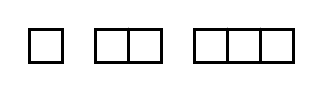
\begin{tikzpicture}[x=.42cm,y=.42cm,line width=1.1pt,line cap=round]
  \foreach \s/\k in {0/1,2/2,5/3}{
    \draw (\s,0) rectangle +(\k,1);
    \foreach \i in {1,...,\k}{\ifnum\i<\k\relax\draw (\s+\i,0) -- (\s+\i,1);\fi}}
\end{tikzpicture}
\begin{enumerate}
  \item Hoeveel lucifers zijn nodig voor 40 vierkanten?
  \item Hoeveel vierkanten kun je leggen met 200 lucifers?
\end{enumerate}
\begin{solution}
\textbf{a.}~121 \quad \textbf{b.}~66
\end{solution}
\begin{fullsolution}
De rij is $4,\ 7,\ 10,\ \ldots$ met $v=3$, dus $u_n=3n+1$.\\
\textbf{a.}~$u_{40}=121$.\\
\textbf{b.}~$3n+1\leqslant 200$ geeft $n\leqslant 66{,}33\ldots$, dus 66 vierkanten (199 lucifers).
\end{fullsolution}
\end{oefening}

\begin{oefening}[2]
\thema{meetkundig: voorschriften}Een bal valt van 2 m hoogte en stuit telkens terug tot 60\% van de vorige hoogte.
\begin{enumerate}
  \item Hoe hoog komt de bal na de 4de keer stuiten?
  \item Na hoeveel keer stuiten komt de bal voor het eerst niet meer boven 5 cm?
\end{enumerate}
\begin{solution}
\textbf{a.}~ongeveer 26 cm \quad \textbf{b.}~8 keer
\end{solution}
\begin{fullsolution}
$u_n=2\cdot 0{,}6^{\,n}$ in m.\\
\textbf{a.}~$u_4=2\cdot 0{,}1296\approx 0{,}26$.\\
\textbf{b.}~$2\cdot 0{,}6^{\,n}\leqslant 0{,}05$ geeft $0{,}6^{\,n}\leqslant 0{,}025$ en $n\geqslant 7{,}22$, dus 8 keer.
\end{fullsolution}
\end{oefening}

\begin{oefening}[2]
\thema{rekenkundig: lineaire groei}De punten $(1, 8)$, $(2, 5)$ en $(3, 2)$ liggen op de grafiek van een rij. Geef het voorschrift. Bij welke $n$ komt het eerste punt onder de $n$-as?
\begin{solution}
$u_n=11-3n$; bij $n=4$
\end{solution}
\begin{fullsolution}
$v=-3$ en $u_1=8$, dus $u_n=11-3n$. $11-3n<0$ geeft $n>3{,}67$, dus $n=4$.
\end{fullsolution}
\end{oefening}

\begin{oefening}[2]
\thema{meetkundig: exponentiële groei}De punten $(1, 3)$, $(2, 6)$ en $(3, 12)$ liggen op de grafiek van een meetkundige rij. Geef het voorschrift. Bij welke $n$ komt de grafiek voor het eerst boven 100?
\begin{solution}
$u_n=3\cdot 2^{n-1}$; bij $n=7$
\end{solution}
\begin{fullsolution}
$q=2$ en $u_1=3$. $3\cdot 2^{n-1}>100$ geeft $n-1>5{,}06$, dus $n=7$ ($u_6=96$ en $u_7=192$).
\end{fullsolution}
\end{oefening}

\begin{oefening}[2]
\thema{rekenkundig: voorschriften}De onderste sport van een ladder zit 30 cm boven de grond. Elke volgende sport zit 28 cm hoger.
\begin{enumerate}
  \item Hoe hoog zit sport 12?
  \item Welke sport zit op 198 cm?
\end{enumerate}
\begin{solution}
\textbf{a.}~338 cm \quad \textbf{b.}~sport 7
\end{solution}
\begin{fullsolution}
\textbf{a.}~$u_{12}=30+11\cdot 28=338$.\\
\textbf{b.}~$30+(n-1)\cdot 28=198$ geeft $n-1=6$, dus $n=7$.
\end{fullsolution}
\end{oefening}

\begin{oefening}[2]
\thema{meetkundig: exponentiële groei}Na inname zit er 200 mg van een medicijn in het bloed. Elk uur wordt 20\% afgebroken.
\begin{enumerate}
  \item Hoeveel zit er nog in het bloed na 5 uur?
  \item Na hoeveel uur is dat voor het eerst minder dan 10 mg?
\end{enumerate}
\begin{solution}
\textbf{a.}~ongeveer 65,5 mg \quad \textbf{b.}~na 14 uur
\end{solution}
\begin{fullsolution}
$u_n=200\cdot 0{,}8^{\,n}$.\\
\textbf{a.}~$u_5=200\cdot 0{,}32768\approx 65{,}5$.\\
\textbf{b.}~$0{,}8^{\,n}<0{,}05$ geeft $n>13{,}43$, dus na 14 uur.
\end{fullsolution}
\end{oefening}

\begin{oefening}[2]
\thema{rekenkundig: term of geen term}Hoeveel positieve termen telt de rij $50,\ 47,\ 44,\ \ldots$?
\begin{solution}
17
\end{solution}
\begin{fullsolution}
$u_n=53-3n>0$ geeft $n<17{,}67$, dus 17 termen. Controle: $u_{17}=2$ en $u_{18}=-1$.
\end{fullsolution}
\end{oefening}

\begin{oefening}[2]
\thema{meetkundig: term of geen term}Welke term van $1000,\ 500,\ 250,\ \ldots$ is de eerste die kleiner is dan 1?
\begin{solution}
$u_{11}\approx 0{,}98$
\end{solution}
\begin{fullsolution}
$1000\cdot(\tfrac12)^{n-1}<1$ geeft $2^{n-1}>1000$ en $n-1>9{,}97$, dus $n=11$ en $u_{11}=\tfrac{1000}{1024}\approx 0{,}98$.
\end{fullsolution}
\end{oefening}

\begin{oefening}[2]
\thema{meetkundig midden}$x - 2$, $x + 1$ en $x + 7$ zijn opeenvolgende termen van een meetkundige rij. Bepaal $x$ en de drie termen.
\begin{solution}
$x=5$; 3, 6, 12
\end{solution}
\begin{fullsolution}
$(x+1)^2=(x-2)(x+7)$ geeft $x^2+2x+1=x^2+5x-14$, dus $x=5$. De termen zijn 3, 6 en 12.
\end{fullsolution}
\end{oefening}

\begin{oefening}[2]
\thema{lineaire en exponentiële groei}Een loon van \eur 2000 stijgt elke maand met \eur 50. Een ander loon van \eur 2000 stijgt elke maand met 2\%. Welk loon is het hoogst na 12 maanden? En na 36 maanden?
\begin{solution}
Na 12 maanden het eerste; na 36 maanden het tweede.
\end{solution}
\begin{fullsolution}
Na 12 maanden: $2000+12\cdot 50=2600$ en $2000\cdot 1{,}02^{12}\approx 2536{,}48$. Na 36 maanden: $2000+36\cdot 50=3800$ en $2000\cdot 1{,}02^{36}\approx 4079{,}77$.
\end{fullsolution}
\end{oefening}

\begin{oefening}[2]
\thema{rekenkundig: lineaire groei}Een tank bevat 45 liter. Per 100 km verbruikt de auto 6 liter. Na hoeveel kilometer zit er nog 9 liter in?
\begin{solution}
600 km
\end{solution}
\begin{fullsolution}
Met $n$ het aantal keer 100 km is $u_n=45-6n$. $45-6n=9$ geeft $n=6$, dus 600 km.
\end{fullsolution}
\end{oefening}

\begin{oefening}[2]
\thema{meetkundig: twee termen}Voeg tussen 3 en 96 vier getallen in, zodat je een meetkundige rij krijgt.
\begin{solution}
6, 12, 24, 48
\end{solution}
\begin{fullsolution}
Met vier getallen ertussen zijn het 5 sprongen: $q^5=\tfrac{96}{3}=32$, dus $q=2$.
\end{fullsolution}
\end{oefening}

\begin{oefening}[2]
\thema{rekenkundig: lineaire groei}Op rekening A staat \eur 200, met elke maand \eur 30 erbij. Op B staat \eur 500, met elke maand \eur 10 erbij. Wanneer staat op beide evenveel? Hoeveel is dat?
\begin{solution}
Na 15 maanden; \eur 650
\end{solution}
\begin{fullsolution}
$200+30n=500+10n$ geeft $n=15$. Dan staat er $200+30\cdot 15=650$ euro op beide.
\end{fullsolution}
\end{oefening}

\begin{oefening}[2]
\thema{rekenkundig: term of geen term}Hoeveel termen telt de rij $15,\ 18,\ 21,\ \ldots,\ 303$?
\begin{solution}
97
\end{solution}
\begin{fullsolution}
$15+(n-1)\cdot 3=303$ geeft $n-1=96$, dus $n=97$. Let op: 96 is het aantal sprongen, niet het aantal termen.
\end{fullsolution}
\end{oefening}

\begin{oefening}[2]
\thema{intrest}\eur 1000 groeit in 2 jaar met samengestelde intrest aan tot \eur 1210. Wat is de intrestvoet?
\begin{solution}
10\%
\end{solution}
\begin{fullsolution}
$(1+\tfrac{p}{100})^2=1{,}21$ geeft $1+\tfrac{p}{100}=1{,}1$, dus $p=10$.
\end{fullsolution}
\end{oefening}

\begin{oefening}[2]
\thema{rekenkundig: twee termen}Voeg tussen 4 en 34 vijf getallen in, zodat je een rekenkundige rij krijgt.
\begin{solution}
9, 14, 19, 24, 29
\end{solution}
\begin{fullsolution}
Met vijf getallen ertussen heeft de rij 7 termen, dus 6 sprongen: $6v=30$ en $v=5$.
\end{fullsolution}
\end{oefening}

\begin{oefening}[2]
\thema{meetkundig: voorschriften}Een blad papier is 0,1 mm dik. Bij elke plooi verdubbelt de dikte.
\begin{enumerate}
  \item Hoe dik is het na 7 plooien?
  \item Hoeveel plooien heb je in theorie nodig om dikker te zijn dan 1 meter?
\end{enumerate}
\begin{solution}
\textbf{a.}~12,8 mm \quad \textbf{b.}~14
\end{solution}
\begin{fullsolution}
$u_n=0{,}1\cdot 2^{\,n}$ in mm.\\
\textbf{a.}~$u_7=0{,}1\cdot 128=12{,}8$.\\
\textbf{b.}~$0{,}1\cdot 2^{\,n}>1000$ geeft $2^{\,n}>10\,000$ en $n>13{,}29$, dus 14 plooien.
\end{fullsolution}
\end{oefening}

\begin{oefening}[2]
\thema{meetkundig: term of geen term}Hoeveel termen telt de rij $5,\ 10,\ 20,\ \ldots,\ 5120$?
\begin{solution}
11
\end{solution}
\begin{fullsolution}
$5\cdot 2^{n-1}=5120$ geeft $2^{n-1}=1024=2^{10}$, dus $n-1=10$ en $n=11$.
\end{fullsolution}
\end{oefening}

\begin{oefening}[2]
\thema{rekenkundig: term of geen term}Welke term van $2,\ 5,\ 8,\ \ldots$ ligt het dichtst bij 1000?
\begin{solution}
$u_{334}=1001$
\end{solution}
\begin{fullsolution}
$u_n=3n-1$. Uit $3n-1=1000$ volgt $n=333{,}67$. Vergelijk: $u_{333}=998$ en $u_{334}=1001$, dus $u_{334}$ ligt het dichtst bij.
\end{fullsolution}
\end{oefening}

\begin{oefening}[2]
\thema{rekenkundig: voorschriften}$u_n = -2n + 9$. Bepaal $u_1$ en $v$. Vanaf welke $n$ zijn de termen negatief?
\begin{solution}
$u_1=7$, $v=-2$; vanaf $n=5$
\end{solution}
\begin{fullsolution}
$u_1=7$ en $v=-2$. $-2n+9<0$ geeft $n>4{,}5$, dus vanaf $n=5$.
\end{fullsolution}
\end{oefening}

\begin{oefening}[2]
\thema{rekenkundig: twee termen}De punten $(2, 5)$ en $(6, 17)$ liggen op de grafiek van een rekenkundige rij. Ligt $(30, 90)$ er ook op?
\begin{solution}
Nee, $u_{30}=89$.
\end{solution}
\begin{fullsolution}
4 sprongen: $4v=12$, dus $v=3$ en $u_1=2$. Dan is $u_{30}=2+29\cdot 3=89$.
\end{fullsolution}
\end{oefening}

\begin{oefening}[2]
\thema{intrest}Hoeveel moet je nu beleggen aan 3\% samengestelde intrest om over 5 jaar \eur 10\,000 te hebben?
\begin{solution}
Ongeveer \eur 8626,09
\end{solution}
\begin{fullsolution}
$K_0\cdot 1{,}03^5=10\,000$ geeft $K_0=\dfrac{10\,000}{1{,}03^5}\approx 8626{,}09$.
\end{fullsolution}
\end{oefening}

\begin{oefening}[3]
\thema{meetkundig: exponentiële groei}Een hoeveelheid daalt met 10\% per jaar. Na hoeveel jaar is ze gehalveerd?
\begin{solution}
Na ongeveer 6,6 jaar
\end{solution}
\begin{fullsolution}
$0{,}9^{\,n}=0{,}5$ geeft $n=\log_{0{,}9} 0{,}5\approx 6{,}6$. Dit hangt niet af van de beginhoeveelheid.
\end{fullsolution}
\end{oefening}

\begin{oefening}[3]
\thema{rekenkundig: term of geen term}Hoeveel getallen van drie cijfers zijn een veelvoud van 7?
\begin{solution}
128
\end{solution}
\begin{fullsolution}
Het kleinste is $105=7\cdot 15$ en het grootste is $994=7\cdot 142$. De rij $105,\ 112,\ \ldots,\ 994$ telt $142-15+1=128$ termen.
\end{fullsolution}
\end{oefening}

\begin{oefening}[3]
\thema{rekenkundig: twee termen}$u_2 + u_4 = 22$ en $u_6 = 23$. Bepaal $u_1$ en $v$.
\begin{solution}
$v=4$, $u_1=3$
\end{solution}
\begin{fullsolution}
$2u_1+4v=22$ en $u_1+5v=23$. Uit de eerste volgt $u_1=11-2v$; invullen geeft $11+3v=23$, dus $v=4$ en $u_1=3$.
\end{fullsolution}
\end{oefening}

\begin{oefening}[3]
\thema{meetkundig midden}Drie opeenvolgende termen van een meetkundige rij hebben als product 216 en als som 19. Welke termen zijn het?
\begin{solution}
4, 6, 9 (of 9, 6, 4)
\end{solution}
\begin{fullsolution}
Noem de termen $\tfrac{a}{q}$, $a$ en $aq$. Het product is $a^3=216$, dus $a=6$. De som geeft $\tfrac6q+6+6q=19$, dus $6q^2-13q+6=0$ en $q=\tfrac32$ of $q=\tfrac23$.
\end{fullsolution}
\end{oefening}

\begin{oefening}[3]
\thema{rekenkundig: voorschriften}Bewijs: als $u_n = pn + q$ met $p$ en $q$ vaste getallen, dan is de rij rekenkundig. Wat is het verschil?
\begin{solution}
Het verschil is $p$.
\end{solution}
\begin{fullsolution}
$u_{n+1}-u_n=p(n+1)+q-(pn+q)=p$. Dit hangt niet af van $n$, dus de rij is rekenkundig met $v=p$.
\end{fullsolution}
\end{oefening}

\begin{oefening}[3]
\thema{rekenkundig midden}Drie opeenvolgende termen van een rekenkundige rij hebben als som 33 en als product 1155. Welke termen zijn het?
\begin{solution}
7, 11, 15 (of 15, 11, 7)
\end{solution}
\begin{fullsolution}
Noem de termen $a-v$, $a$ en $a+v$. De som is $3a=33$, dus $a=11$. Het product is $11(121-v^2)=1155$, dus $v^2=16$ en $v=\pm 4$.
\end{fullsolution}
\end{oefening}

\begin{oefening}[3]
\thema{meetkundig: voorschriften}Bewijs: als $u_n = a \cdot b^{\,n}$ met $a$ en $b$ vaste getallen verschillend van 0, dan is de rij meetkundig. Wat is het quotiënt?
\begin{solution}
Het quotiënt is $b$.
\end{solution}
\begin{fullsolution}
$\dfrac{u_{n+1}}{u_n}=\dfrac{a\cdot b^{\,n+1}}{a\cdot b^{\,n}}=b$. Dit hangt niet af van $n$, dus de rij is meetkundig met $q=b$.
\end{fullsolution}
\end{oefening}

\end{oefeningen}

%----------------------------------------------------------------------------------------
% KOPPEL: verbanden met andere leerstof. Enkel waar het zinvol is; geen koppeling tussen
% leerstof die vanzelf uit elkaar volgt (zoals limieten, afgeleiden en integralen).
%----------------------------------------------------------------------------------------
\opdrachtsectie{Koppel}

\lkr{Kijk na of deze leerstof al gezien is in jouw jaarplanning. Kansrekenen staat bv. ook in het 6de jaar.}

\begin{oefeningen}
\begin{oefening}[2]
\koppel{analyse}{Exponentiële functies} Gegeven: $f(x) = 5 \cdot 2^{\,x}$.
\begin{enumerate}
  \item Bereken $f(1)$, $f(2)$, $f(3)$ en $f(4)$. Welke soort rij vormen die getallen? Wat is het quotiënt?
  \item Wat is het quotiënt als je alleen $f(1)$, $f(3)$, $f(5)$, \ldots\ neemt?
\end{enumerate}
\begin{solution}
\textbf{a.}~10, 20, 40, 80; meetkundig, $q=2$ \quad \textbf{b.}~$q=4$
\end{solution}
\begin{fullsolution}
\textbf{a.}~Elke stap van 1 in $x$ vermenigvuldigt met 2, dus $q=2$.\\
\textbf{b.}~$\dfrac{f(3)}{f(1)}=2^2=4$.
\end{fullsolution}
\end{oefening}

\begin{oefening}[3]
\koppel{analyse}{Logaritmen} Gegeven is de meetkundige rij $2,\ 8,\ 32,\ 128,\ \ldots$
\begin{enumerate}
  \item Bereken $\log_2$ van elke term. Welke soort rij krijg je?
  \item Toon aan: de logaritmen van de termen van een meetkundige rij met positieve termen vormen een rekenkundige rij. Wat is het verschil?
\end{enumerate}
\begin{solution}
\textbf{a.}~1, 3, 5, 7; rekenkundig, $v=2$ \quad \textbf{b.}~$v=\log q$
\end{solution}
\begin{fullsolution}
\textbf{a.}~$\log_2 2=1$, $\log_2 8=3$, $\log_2 32=5$, $\log_2 128=7$.\\
\textbf{b.}~$\log u_n=\log\left(u_1 q^{\,n-1}\right)=\log u_1+(n-1)\log q$. Dit is een rekenkundige rij met eerste term $\log u_1$ en verschil $\log q$.
\end{fullsolution}
\end{oefening}

\begin{oefening}[2]
\koppel{algebra}{Matrices} Gegeven: $A = \begin{pmatrix} 1 & 2 \\ 0 & 1 \end{pmatrix}$.
\begin{enumerate}
  \item Bereken $A^2$ en $A^3$. Welke rij vormen de elementen rechtsboven in $A$, $A^2$, $A^3$?
  \item Bepaal $A^{10}$ zonder verder te vermenigvuldigen.
\end{enumerate}
\begin{solution}
\textbf{a.}~Rechtsboven: 2, 4, 6; rekenkundig, $v=2$ \quad \textbf{b.}~$A^{10}=\begin{pmatrix} 1 & 20 \\ 0 & 1 \end{pmatrix}$
\end{solution}
\begin{fullsolution}
\textbf{a.}~$A^2=\begin{pmatrix} 1 & 4 \\ 0 & 1 \end{pmatrix}$ en $A^3=\begin{pmatrix} 1 & 6 \\ 0 & 1 \end{pmatrix}$.\\
\textbf{b.}~Het element rechtsboven is $u_n=2n$, dus $u_{10}=20$.
\end{fullsolution}
\end{oefening}

\begin{oefening}[2]
\koppel{algebra}{Complexe getallen} Gegeven: $u_n = (1 + \mathrm{i})^n$.
\begin{enumerate}
  \item Bereken $u_1$, $u_2$, $u_3$ en $u_4$. Wat is het quotiënt van deze rij?
  \item Welke rij vormen de moduli van deze termen?
\end{enumerate}
\begin{solution}
\textbf{a.}~$1+\mathrm{i}$, $2\mathrm{i}$, $-2+2\mathrm{i}$, $-4$; $q=1+\mathrm{i}$ \quad \textbf{b.}~meetkundig, $q=\sqrt2$
\end{solution}
\begin{fullsolution}
\textbf{a.}~Telkens vermenigvuldigen met $1+\mathrm{i}$: $(1+\mathrm{i})^2=2\mathrm{i}$, $2\mathrm{i}(1+\mathrm{i})=-2+2\mathrm{i}$, $(2\mathrm{i})^2=-4$.\\
\textbf{b.}~De moduli zijn $\sqrt2$, $2$, $2\sqrt2$, $4$: telkens maal $\sqrt2$.
\end{fullsolution}
\end{oefening}

\needspace{14\baselineskip}% figuur en deelvragen bij de opgave houden
\begin{oefening}[2]
\koppel{meetkunde}{Vlakke meetkunde} Een vierkant heeft een oppervlakte van 16 cm\textsuperscript{2}. Door de middens van de zijden te verbinden, krijg je een nieuw vierkant, enzovoort.

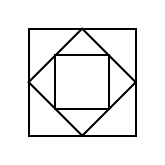
\begin{tikzpicture}[scale=.34,line width=.7pt]
  \draw (0,0) -- (4,0) -- (4,4) -- (0,4) -- cycle;
  \draw (2,0) -- (4,2) -- (2,4) -- (0,2) -- cycle;
  \draw (1,1) -- (3,1) -- (3,3) -- (1,3) -- cycle;
\end{tikzpicture}
\begin{enumerate}
  \item Toon aan dat de oppervlakte telkens halveert.
  \item Wat is de oppervlakte van het 6de vierkant?
\end{enumerate}
\begin{solution}
\textbf{b.}~$\tfrac12$ cm\textsuperscript{2}
\end{solution}
\begin{fullsolution}
\textbf{a.}~De vier hoekdriehoeken die wegvallen, zijn samen even groot als het nieuwe vierkant. De oppervlakte halveert dus: $q=\tfrac12$.\\
\textbf{b.}~$u_6=16\cdot(\tfrac12)^5=\tfrac12$.
\end{fullsolution}
\end{oefening}

\begin{oefening}[2]
\begin{metprent}{dobbelstenen}
\koppel{data}{Kansrekenen} Je gooit met een dobbelsteen tot je een zes gooit.
\begin{enumerate}
  \item Bereken de kans dat de eerste zes valt bij worp 1, worp 2 en worp 3. Welke soort rij is dat?
  \item Vanaf welke worp is die kans kleiner dan 1\%?
\end{enumerate}
\end{metprent}
\begin{solution}
\textbf{a.}~$\tfrac16$, $\tfrac{5}{36}$, $\tfrac{25}{216}$; meetkundig, $q=\tfrac56$ \quad \textbf{b.}~vanaf worp 17
\end{solution}
\begin{fullsolution}
\textbf{a.}~Eerst $n-1$ keer geen zes, dan wel een zes: $u_n=\tfrac16\cdot(\tfrac56)^{n-1}$.\\
\textbf{b.}~$\tfrac16\cdot(\tfrac56)^{n-1}<0{,}01$ geeft $(\tfrac56)^{n-1}<0{,}06$ en $n-1>15{,}43$, dus $n=17$.
\end{fullsolution}
\end{oefening}
\end{oefeningen}

%----------------------------------------------------------------------------------------
\opdrachtsectie{Test jezelf}

\begin{oefeningen}
\begin{oefening}\label{oef:t1}
Is de rij rekenkundig, meetkundig of geen van beide? Geef $v$ of $q$.
\begin{reeks}
  \item $11,\ 8,\ 5,\ 2,\ \ldots$
  \item $3,\ {-6},\ 12,\ {-24},\ \ldots$
  \item $1,\ 2,\ 4,\ 7,\ \ldots$
\end{reeks}
\begin{solution}
\textbf{a.}~rekenkundig, $v=-3$ \quad \textbf{b.}~meetkundig, $q=-2$ \quad \textbf{c.}~geen van beide
\end{solution}
\begin{fullsolution}
\textbf{a.}~Telkens $-3$.\\
\textbf{b.}~Telkens maal $-2$.\\
\textbf{c.}~Verschillen 1, 2, 3 en quotiënten 2, 2, $\tfrac74$: niet constant.
\end{fullsolution}
\end{oefening}

\begin{oefening}\label{oef:t2}
Geef een recursief en een expliciet voorschrift van $4,\ 10,\ 16,\ \ldots$
\begin{solution}
$u_n=u_{n-1}+6$, $u_1=4$; $u_n=6n-2$
\end{solution}
\begin{fullsolution}
$v=6$, dus $u_n=u_{n-1}+6$ met $u_1=4$, en $u_n=4+(n-1)\cdot 6=6n-2$.
\end{fullsolution}
\end{oefening}

\begin{oefening}\label{oef:t3}
Geef een recursief en een expliciet voorschrift van $2,\ 10,\ 50,\ \ldots$
\begin{solution}
$u_n=5u_{n-1}$, $u_1=2$; $u_n=2\cdot 5^{n-1}$
\end{solution}
\begin{fullsolution}
$q=5$, dus $u_n=5u_{n-1}$ met $u_1=2$, en $u_n=2\cdot 5^{n-1}$.
\end{fullsolution}
\end{oefening}

\begin{oefening}\label{oef:t4}
Een rekenkundige rij heeft $u_4 = 13$ en $u_{11} = 41$. Bepaal $u_1$ en $v$.
\begin{solution}
$v=4$, $u_1=1$
\end{solution}
\begin{fullsolution}
7 sprongen: $7v=28$, dus $v=4$. Drie sprongen terug: $u_1=13-3\cdot 4=1$.
\end{fullsolution}
\end{oefening}

\begin{oefening}\label{oef:t5}
Een meetkundige rij heeft $u_2 = 6$ en $u_5 = 48$. Bepaal $u_1$ en $q$.
\begin{solution}
$q=2$, $u_1=3$
\end{solution}
\begin{fullsolution}
3 sprongen: $q^3=8$, dus $q=2$. Een sprong terug: $u_1=\tfrac62=3$.
\end{fullsolution}
\end{oefening}

\begin{oefening}\label{oef:t6}
Is 100 een term van $4,\ 10,\ 16,\ \ldots$? En 101?
\begin{solution}
100 is de 17de term; 101 is geen term.
\end{solution}
\begin{fullsolution}
$6n-2=100$ geeft $n=17$. $6n-2=101$ geeft $n=\tfrac{103}{6}$: geen natuurlijk getal.
\end{fullsolution}
\end{oefening}

\begin{oefening}\label{oef:t7}
Is 1024 een term van $2,\ 4,\ 8,\ \ldots$? En 1000?
\begin{solution}
1024 is de 10de term; 1000 is geen term.
\end{solution}
\begin{fullsolution}
$u_n=2^{\,n}$. $2^{\,n}=1024$ geeft $n=10$. $2^{\,n}=1000$ geeft $n\approx 9{,}97$: geen natuurlijk getal.
\end{fullsolution}
\end{oefening}

\begin{oefening}\label{oef:t8}
Een kaars is 30 cm lang en brandt 1,5 cm per uur op. Geef een voorschrift voor de lengte na $n$ uur. Wanneer is de kaars op?
\begin{solution}
$u_n=30-1{,}5\,n$; na 20 uur
\end{solution}
\begin{fullsolution}
$u_0=30$ en $v=-1{,}5$, dus $u_n=30-1{,}5\,n$. Uit $u_n=0$ volgt $n=20$.
\end{fullsolution}
\end{oefening}

\begin{oefening}\label{oef:t9}
Je belegt \eur 4000 aan 2\% samengestelde intrest. Hoeveel heb je na 5 jaar?
\begin{solution}
Ongeveer \eur 4416,32
\end{solution}
\begin{fullsolution}
$K_5=4000\cdot 1{,}02^5\approx 4416{,}32$.
\end{fullsolution}
\end{oefening}
\end{oefeningen}

\herhaalschema{%
  \fzv{oef:t1}{oef:soort}%
  \fv{oef:t2}{vb:term}{oef:voorschrift}%
  \fv{oef:t3}{vb:mterm}{oef:mvoorschrift}%
  \fv{oef:t4}{vb:tweetermen}{oef:tweetermen}%
  \fv{oef:t5}{vb:mtwee}{oef:mtwee}%
  \fv{oef:t6}{vb:isterm}{oef:isterm}%
  \fv{oef:t7}{vb:misterm}{oef:misterm}%
  \fv{oef:t8}{vb:groei}{oef:groei}%
  \fv{oef:t9}{vb:intrest}{oef:intrest}}

\ifzelfstudie
\section*{Maak je eigen samenvatting}
Sluit dit boek en schrijf in je schrift: wat is een rekenkundige en wat is een meetkundige rij, welke voorschriften horen erbij, hoe vind je de rij uit twee termen, hoe test je of een getal een term is, wat is het verschil tussen enkelvoudige en samengestelde intrest, en welke fouten wil je vermijden? Vergelijk daarna met de kaders.
\fi
